\documentclass[tikz,border=0pt]{standalone}
\usepackage[american]{circuitikz}
\usetikzlibrary{arrows.meta,calc,positioning,decorations.pathmorphing,patterns}
\definecolor{zyloTeal}{HTML}{174A5B}
\definecolor{zyloTealTwo}{HTML}{246B7A}
\definecolor{zyloInk}{HTML}{1F2933}
\definecolor{zyloSoft}{HTML}{EAF4F4}
\definecolor{zyloPaper}{HTML}{F8FAFB}
\definecolor{zyloLine}{HTML}{44606B}
\definecolor{zyloOrange}{HTML}{D97706}
\begin{document}
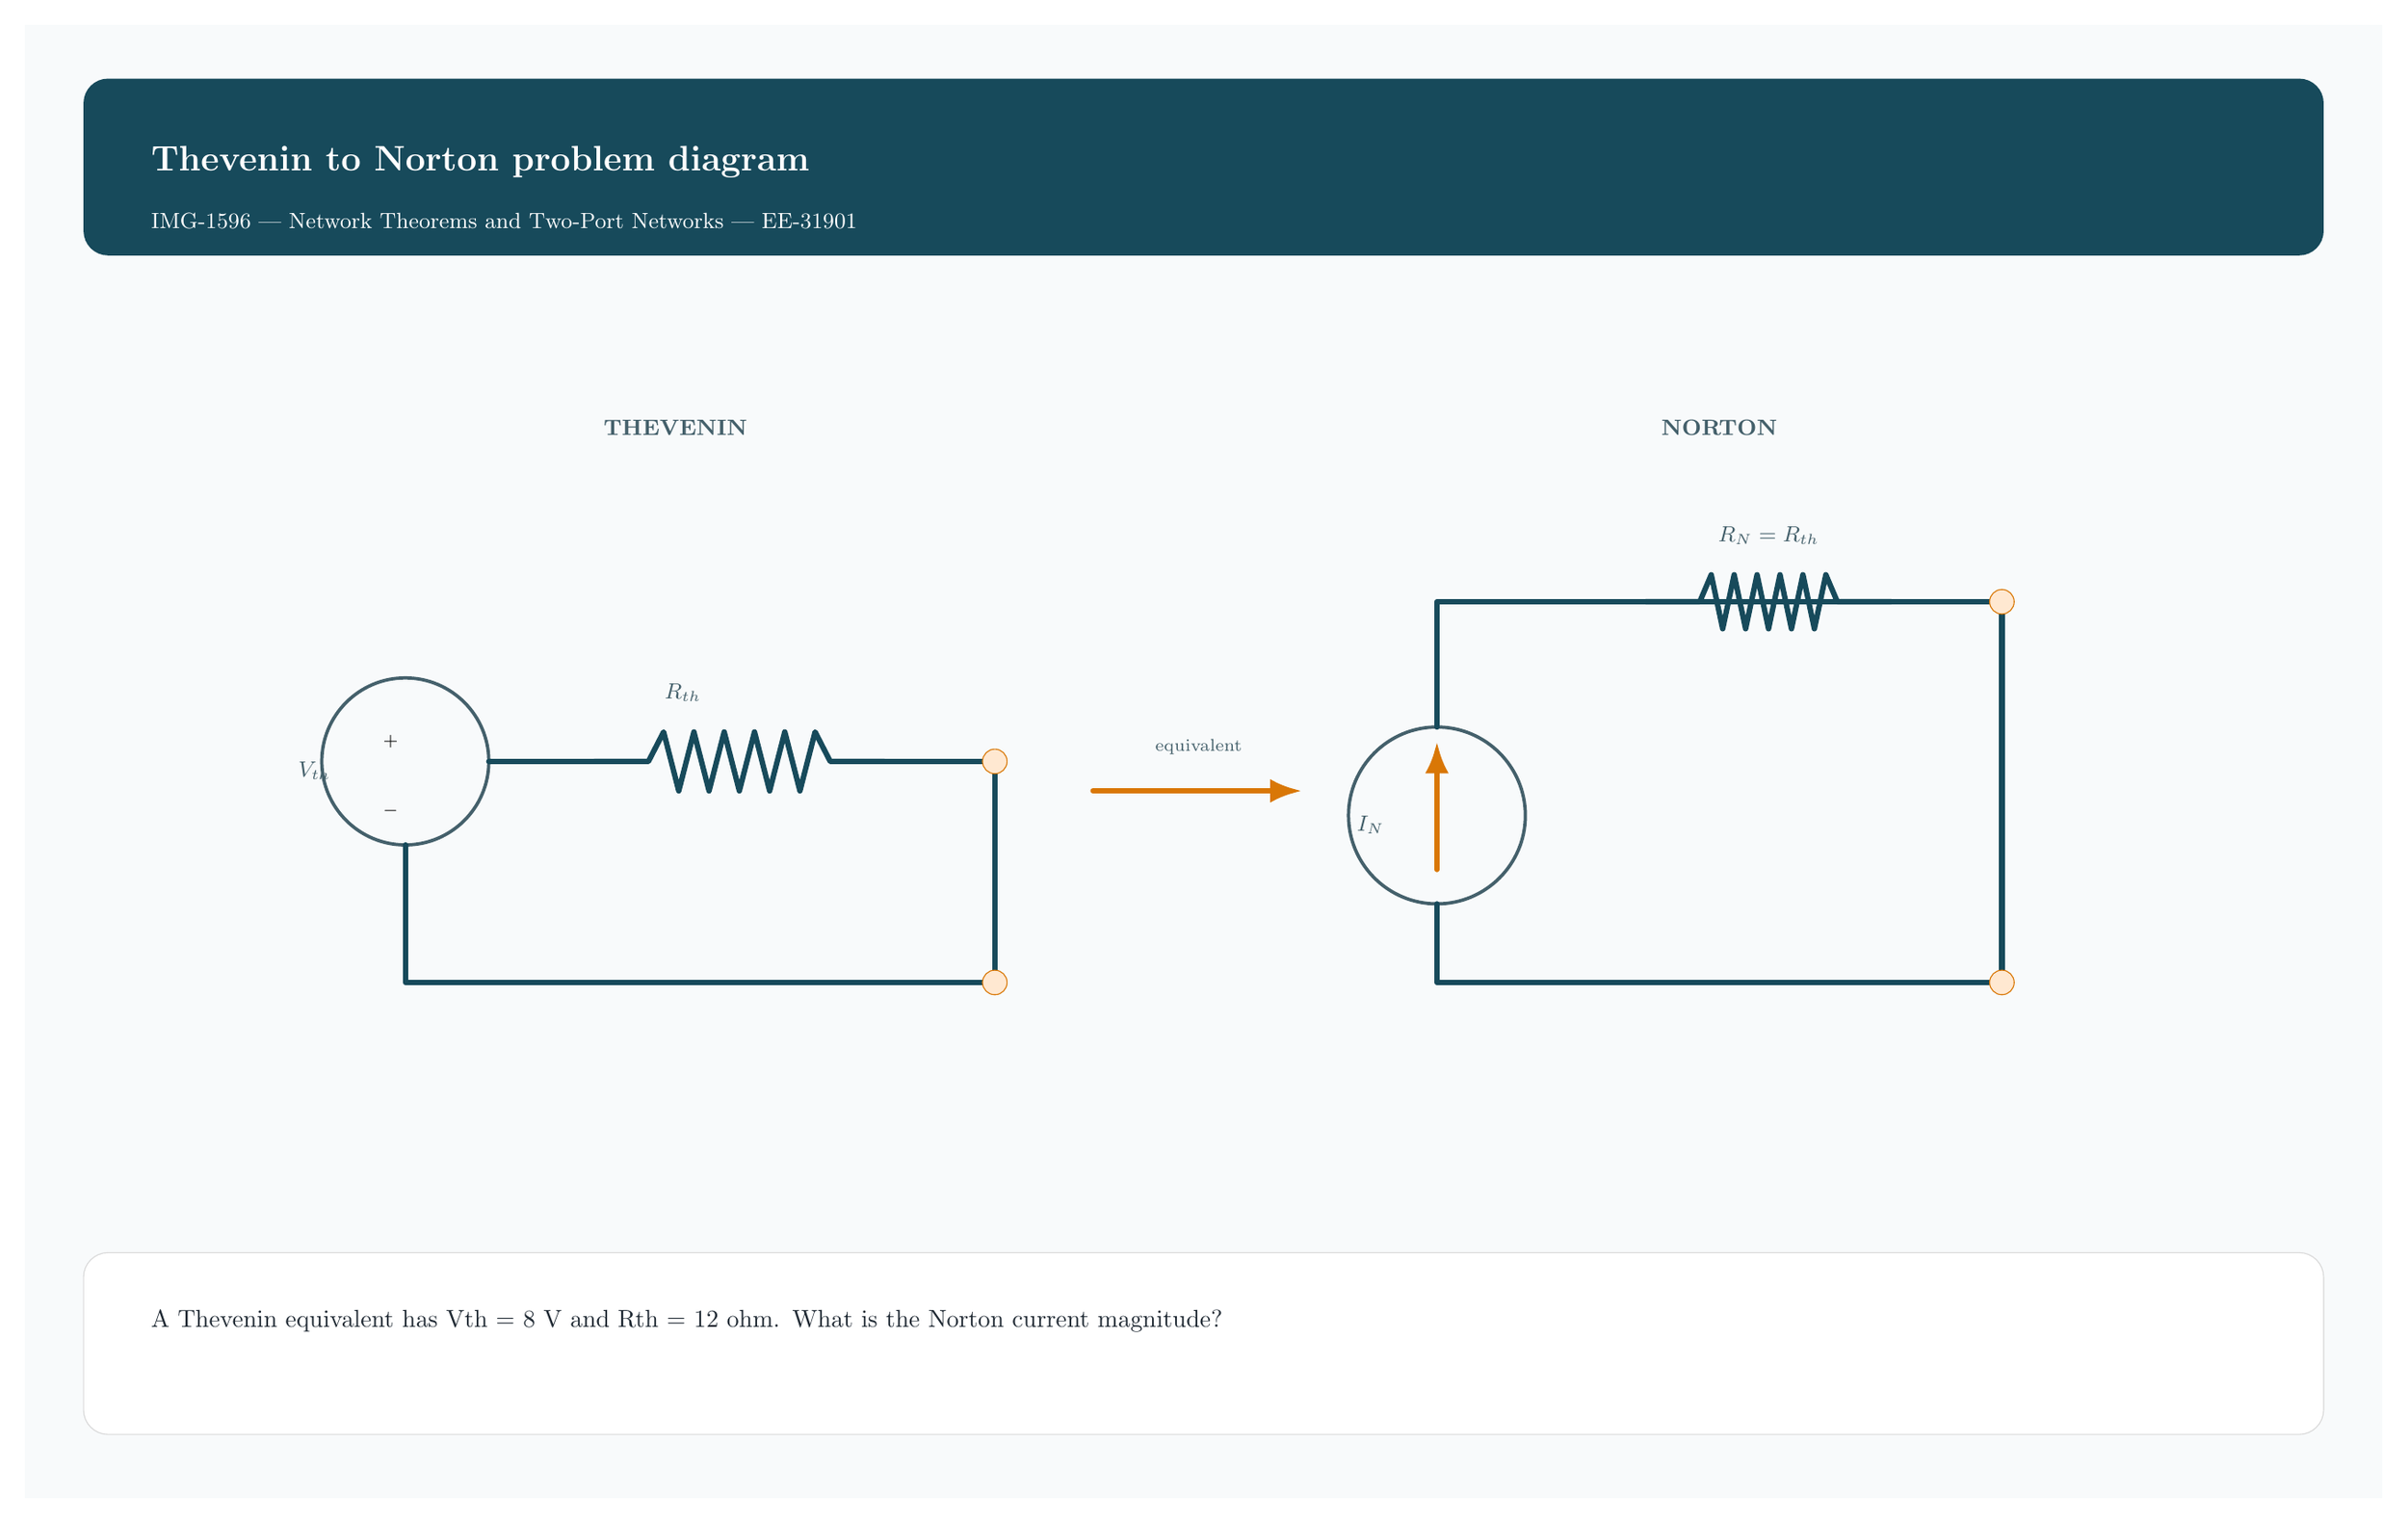
\begin{tikzpicture}[x=1pt,y=-1pt,>=Latex,line cap=round,line join=round]
\path[fill=zyloPaper] (0,0) rectangle (960,600);
\path[fill=zyloTeal,rounded corners=10pt] (24,22) rectangle (936,94);
\node[anchor=west,text=white,font=\bfseries\Large] at (48,56) {Thevenin to Norton problem diagram};
\node[anchor=west,text=white!82,font=\small] at (48,80) {IMG-1596 | Network Theorems and Two-Port Networks | EE-31901};
\tikzset{wire/.style={draw=zyloTeal,line width=2.2pt},thinwire/.style={draw=zyloLine,line width=1.35pt},accent/.style={draw=zyloOrange,line width=2.2pt},box/.style={draw=zyloTealTwo,fill=zyloSoft,line width=1.5pt,rounded corners=8pt}}
\node[font=\small\bfseries,text=zyloLine] at (265,164) {THEVENIN};
\draw[thinwire] (155,300) circle (34); \node[font=\scriptsize] at (149,292) {$+$}; \node[font=\scriptsize] at (149,320) {$-$};
\draw[wire] (189,300) -- (232,300);
\draw[wire] (232,300) -- (254,300) -- (254,300) -- (260.167,288) -- (266.333,312) -- (272.5,288) -- (278.667,312) -- (284.833,288) -- (291,312) -- (297.167,288) -- (303.333,312) -- (309.5,288) -- (315.667,312) -- (321.833,288) -- (328,300) -- (350,300);
\draw[wire] (350,300) -- (395,300); \draw[wire] (395,300) -- (395,390) -- (155,390) -- (155,334);
\filldraw[draw=zyloOrange,fill=orange!18] (395,300) circle (5); \filldraw[draw=zyloOrange,fill=orange!18] (395,390) circle (5);
\node[font=\small,text=zyloLine] at (268,272) {$R_{th}$}; \node[font=\small,text=zyloLine] at (118,304) {$V_{th}$};
\node[font=\small\bfseries,text=zyloLine] at (690,164) {NORTON};
\draw[thinwire] (575,322) circle (36); \draw[accent,->] (575,344) -- (575,292);
\draw[wire] (575,286) -- (575,235) -- (805,235) -- (805,390) -- (575,390) -- (575,358);
\draw[wire] (660,235) -- (682,235) -- (682,235) -- (686.667,224) -- (691.333,246) -- (696,224) -- (700.667,246) -- (705.333,224) -- (710,246) -- (714.667,224) -- (719.333,246) -- (724,224) -- (728.667,246) -- (733.333,224) -- (738,235) -- (760,235);
\filldraw[draw=zyloOrange,fill=orange!18] (805,235) circle (5); \filldraw[draw=zyloOrange,fill=orange!18] (805,390) circle (5);
\node[font=\small,text=zyloLine] at (710,208) {$R_N=R_{th}$}; \node[font=\small,text=zyloLine] at (548,326) {$I_N$};
\draw[accent,->] (435,312) -- (520,312); \node[font=\scriptsize,text=zyloLine] at (478,294) {equivalent};
\path[draw=black!15,fill=white,rounded corners=10pt] (24,500) rectangle (936,574);
\node[anchor=west,text width=860pt,align=left,text=zyloInk,font=\normalsize] at (48,528) {A Thevenin equivalent has Vth = 8 V and Rth = 12 ohm. What is the Norton current magnitude?};
\end{tikzpicture}
\end{document}
